\begin{enumerate}
\item On considère la fonction $g$ définie sur l'intervalle $[0~;~2\pi]$ par :
\[
g(x)=x\cos(x)-\sin(x)
\]

On admet que la fonction $g$ est dérivable sur l'intervalle $[0~;~2\pi]$ et on note $g'$ sa dérivée.

\begin{enumerate}
\item Montrer que pour tout réel $x$ de l'intervalle $[0~;~2\pi]$, on a :
\[
g'(x)=-x\sin(x)
\]

\item On donne le tableau de variations de la fonction $g$ sur l'intervalle $[0~;~2\pi]$ ci-dessous.

Justifier chacun des éléments qui figurent dans ce tableau de variations.

\begin{center}
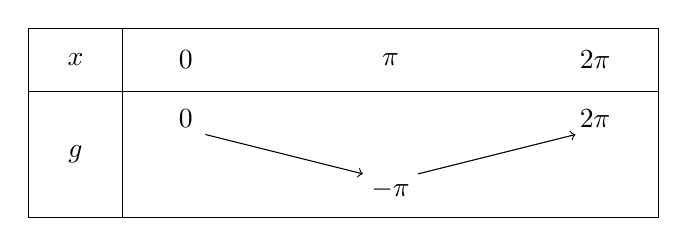
\begin{tikzpicture}[x=1cm,y=1cm]
\draw (0,0) rectangle (8,2.4);
\draw (1.2,0) -- (1.2,2.4);
\draw (0,1.6) -- (8,1.6);
\node at (0.6,2) {$x$};
\node at (2,2) {$0$};
\node at (4.6,2) {$\pi$};
\node at (7.2,2) {$2\pi$};
\node at (0.6,0.8) {$g$};
\node at (2,1.25) {$0$};
\node at (4.6,0.35) {$-\pi$};
\node at (7.2,1.25) {$2\pi$};
\draw[->] (2.25,1.05) -- (4.25,0.55);
\draw[->] (4.95,0.55) -- (6.95,1.05);
\end{tikzpicture}
\end{center}

\item Montrer qu'il existe une unique valeur réelle $\alpha$ dans l'intervalle $[\pi~;~2\pi]$ telle que $g(\alpha)=0$.

\item En déduire le tableau de signes de la fonction $g$ sur l'intervalle $[0~;~2\pi]$.
\end{enumerate}

\item On considère la fonction $f$ définie sur l'intervalle $]0~;~2\pi]$ par :
\[
f(x)=\dfrac{\sin(x)}{x}
\]

On admet que la fonction $f$ est dérivable sur l'intervalle $]0~;~2\pi]$ et on note $f'$ sa dérivée.

\begin{enumerate}
\item Montrer que pour tout réel $x$ de l'intervalle $]0~;~2\pi]$ on a :
\[
f'(x)=\dfrac{g(x)}{x^2}
\]

\item Étudier le signe de la fonction $f'$ sur l'intervalle $]0~;~2\pi]$.

\item En déduire le sens de variation de la fonction $f$ sur l'intervalle $]0~;~2\pi]$.

\item Déterminer la limite de $f$ en $0$. On pourra utiliser le taux d'accroissement de la fonction sinus en $0$.
\end{enumerate}

\item On considère deux nombres réels $r$ et $s$ qui vérifient l'inégalité : $0 < r < s < \pi$.

Montrer que :
\[
\dfrac{r}{s}<\dfrac{\sin(r)}{\sin(s)}
\]
\end{enumerate}
